\begin{frame}{Metal-as-a-Service: MaaS}
    \begin{block}{Bare metal cloud}
        Bare metal cloud is an environment in which physical, dedicated servers can be provisioned to customers with cloud-like ease and speed. \linebreak
        \linebreak
        Bare metal cloud customers are given access to the entire processing power of individual servers, as well as any storage, networking or other services they require.
    \end{block}
\end{frame}

% \begin{frame}{IaaS vs. MaaS}

%     \begin{center}
%         Is there any difference between IaaS \& MaaS?
%     \end{center}

% \end{frame}

% \begin{frame}{IaaS vs. MaaS}

%     \begin{center}
%         This depends on the view point.
%     \end{center}

% \end{frame}

% \begin{frame}{IaaS vs. MaaS}

%     \begin{center}
%         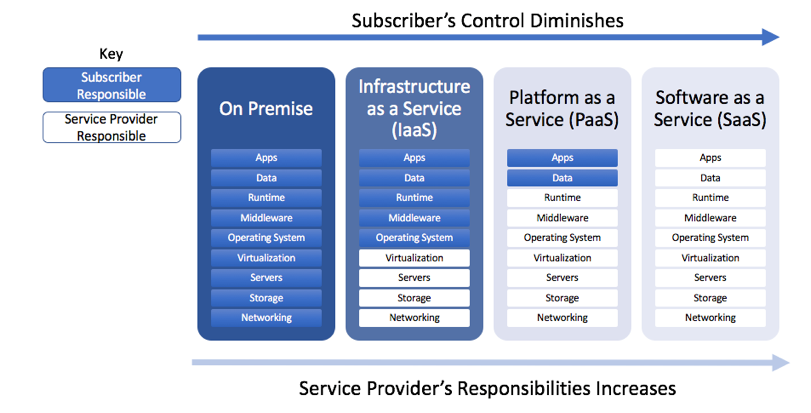
\includegraphics{img/cloud-services-model.png}
%     \end{center}

% \end{frame}

% \begin{frame}{IaaS vs. MaaS}

%     Many define IaaS as the provision of virtual resources only. Some include dedicated servers in their definition.\\

%     \vspace*{0.35cm}

%     On a virtual IaaS, one has no knowledge of or control over the actual infrastructure on which your services are built. The provider has control of these and your services are abstracted from them.\\

%     \vspace*{0.35cm}

%     With bare metal you get control of the full stack, from the tin right up to the user interface, and can optimise utilisation and performance to a granular level, something you simple cannot do in a virtualised environment.

% \end{frame}